\glsresetall

\chapter{Referencial Teórico}
\label{chap.background}

Neste capítulo serão apresentados conceitos fundamentais para o entendimento do trabalho. A \autoref{sec.lw} apresenta uma visão geral da evolução dos processadores, partindo dos \singlecores até os \lws. A \autoref{sec.nanvixos} apresenta o \nanvix, \so que será utilizado no desenvolvimento deste trabalho. A \autoref{sec.virtualizacao} descreve detalhes importantes sobre a virtualização e migração de processos.

\section{Dos \singlecores aos \Lws}
\label{sec.lw}

O aumento de desempenho dos sistemas computacionais manteve-se como uma necessidade constante para o avanço da ciência em vários setores: astrologia, biologia, engenharia, etc. Até tempos atrás, esse objetivo era alcançado através do aumento da frequência de relógios do núcleo de processamento, do avanço na tecnologia dos semicondutores e do acréscimo do número de transistores em um \chip. Atualmente, nós estamos chegando ao limite físico que impede a aplicação de parte dessas técnicas. Além da dificuldade de garantir a dissipação de calor à medida que a frequência aumenta, o número de transistores que conseguimos colocar em uma mesma área de um \chip está chegando ao seu limite físico, \ie o tamanho dos transitores alcançou a escala atômica.

Como alternativa para a continuidade nos avanços de poder computacional, foram exploradas novas técnicas. Em especial, foram desenvolvidas arquiteturas paralelas, que exploram o poder de processamento paralelo, o qual é atingido pela execução de múltiplos \cores simultaneamente. Essas novas arquiteturas são classificadas de acordo com a maneira com que conseguem manipular os dados. São elas:
\begin{inlinelist}
    \item \sisd;
    \item \simd;
    \item \misd;
    \item \mimd.
\end{inlinelist}
Neste trabalho, estamos interessados nas arquiteturas que suportam cargas de trabalho \mimd, as quais ainda podem ser divididas em multiprocessadores ou multicomputadores, como mostrado na \autoref{fig.mimd}~\cite{tanenbaum:4ed}.
% \todo{Sobre a fig mimd, não precisa ser agora mas: mudar o texto nas imagens para pt-br}

Neste contexto, a classe de processadores \lws destacam-se por atrelar alto poder de processamento paralelo com eficiência energética. Os \lws são classificados como \mpsoc e suas arquiteturas apresentam as seguintes características:
\begin{enumerate}[label=(\roman*)]
    \item Integrar de centenas à milhares de núcleos de processamento operando a baixas frequências em um único \chip;
    \item Processar cargas de trabalho \mimd;
    \item Organizar os núcleos em conjuntos, denominados \clusters, para compartilhamento de recursos locais;
    \item Utilizar \nocs para transferência de dados entre núcleos ou \clusters;
    \item Possuir sistemas memória distribuída restritivos, compostos por pequenas memórias locais; e
    \item Apresentar componentes heterogêneos (\cclusters e \ioclusters).
\end{enumerate}

\begin{figure}[t]
    \centering
    \includesvg[width=0.9\linewidth]{content/images/mimd.svg}
    \caption{(a) um multiprocessador de memória compartilhada. (b) um multicomputator com troca de mensagens. (c) um sistema distribuído de grande escala~\cite{tanenbaum:4ed}.}
    \label{fig.mimd}
\end{figure}

Alguns exemplos comerciais bem sucedidos de \lws são o \mppa~\cite{dinechin:2013}, PULP~\cite{pulp} e \taihulight~\cite{fu2016sunway}.
%
Especificamente, para o desenvolvimento deste trabalho foi utilizado o processador \mppa. A \autoref{fig.arch-mppa} apresenta uma visão geral do processador e suas peculiaridades, tais como:

\begin{enumerate}[label=(\roman*)]
    \item Integrar 288 núcleos de baixa frequência em um único \textit{chip};
    \item Possuir núcleos organizados em 20 \clusters;
    \item Dispor de 2 \nocs para transferência de dados entre \clusters, uma para controle e outra para dados;
    \item Possuir um sistema de memória distribuída composto por pequenas memórias locais, \eg \sram de 2 MB;
    \item Não dispor de coerência de \cache;
    \item Apresentar heterogeneidade: \clusters destinados à computação (\cclusters) e \clusters destinados à comunicação com periféricos (\ioclusters).
\end{enumerate}

\begin{figure}[t]
    \centering
    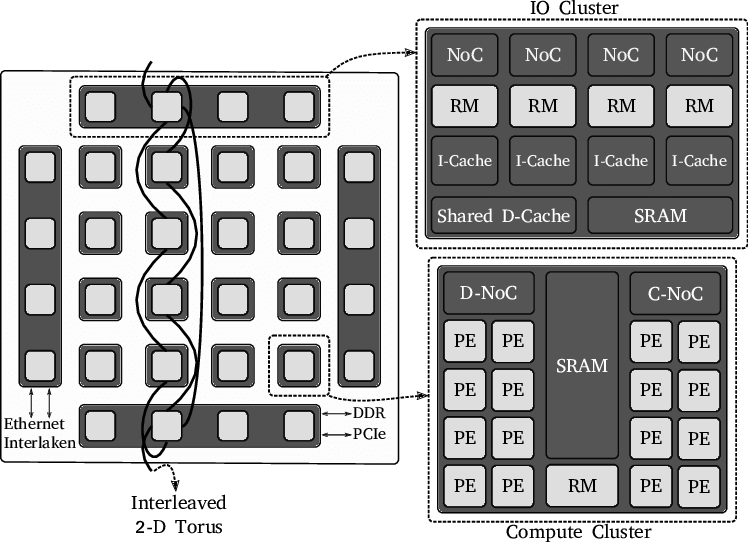
\includegraphics[width=0.6\linewidth]{content/images/arch-mppa-gs.png}
    \caption{Visão arquitetural do processador \mppa~\cite{penna:sbesc19}.}
    \label{fig.arch-mppa}
\end{figure}

\section{\nanvixos}
\label{sec.nanvixos}

O \nanvix\footnote{Disponível em https://github.com/nanvix} é um \os distribuído e de propósito geral que busca equilibrar desempenho, portabilidade e programabilidade para \lws~\cite{penna:sbesc19}. O \nanvix é estruturado em três camadas de \kernel. São elas:
\begin{description}
    \item [\nanvix \hal]
         é a camada mais baixa que abstrai e provê o gerenciamento dos recursos de \hardware sobre uma visão comum~\cite{penna:hal}. Entre esses recursos estão: \cores, \tlbs, \cache, \mmu, \noc, interrupções, memória virtual e recursos de \io. De maneira geral, esta camada provê abstrações ao nivel do \core, \cluster e comunicação/sincronização entre \clusters~\cite{penna:thesis}. A Figura \ref{fig.hal-overview} ilustra a estrutura interna da \hal do \nanvix.
    \item [\nanvix \Microkernel]
        é a camada intermediária que provê gerenciamento de recursos e os serviços mínimos de um \os em um \cluster. Entre esses serviços se encontram a comunição entre processos, gerenciamento de \threads e memória, controle de acesso à memória e interface para chamadas de sistema. As chamadas de sistema podem ser executadas localmente, caso acessem dados \rdo ou alterem estruturas internas do \core, ou remotamente pelo \mcore, que atende à requisição e libera o \score requisitante ao término da chamada~\cite{penna:thesis}. Essa característica adjetiva o \microkernel como assimétrico. A Figura \ref{fig.microkernel-overview} ilustra a estrutura interna do \microkernel do \nanvix.
    \item [\nanvix \Multikernel]
        é a camada superior que provê os serviços mais complexos de um \os e dispõe uma visão a nível do processador em si. Os serviços são hospedados em \ioclusters, \ie isolados das aplicações de usuário. Os serviços atendem as requisições vindas dos processos de usuário através de um modelo cliente-servidor. As requisições e respostas são enviadas/recebidas através de passagem de mensagem via \noc. Os serviços dessa camada podem ser entendidos como fontes de informação que mantém a execução dos processos consistentes no processador, tendo em vista a natureza distribuída da memória nessas arquiteturas. Alguns serviços incluídos no \nanvix são mecanismos de \spawn de processos e gerenciamento de nomes lógicos dos processos à fim a localização dos processos no processador.
\end{description}

\begin{figure}[t]
    \centering
    \includesvg[width=0.8\linewidth]{content/images/hal.svg}
    \caption{Estrutura interna da \hal do \nanvix~\cite{penna:thesis}.}
    \label{fig.hal-overview}
\end{figure}

\begin{figure}[t]
    \centering
    \includesvg[width=0.8\linewidth]{content/images/microkernel.svg}
    \caption{Estrutura interna do \microkernel do \nanvix~\cite{penna:thesis}.}
    \label{fig.microkernel-overview}
\end{figure}

Em sua abordagem original, os processos no \nanvix são estáticos, \ie cada \cluster possui apenas um processo. Desse modo, uma vez que o processo inicia sua execução em um \cluster, este finalizará a execução no mesmo \cluster. 
Isso torna o processo dependente do \cluster que o executa, fazendo com que a comunicação entre processos esteja atrelada aos \clusters nos quais os processos são executados (e não aos processos em si). A falta de mobilidade dos processos nesse modelo pode trazer sobrecargas ao processador, afetando diretamente o o desempenho do sistema quando múltiplas aplicações estão em execução simultânea no processador. No caso de aplicações paralelas, compostas por múltiplos processos (ou \textit{threads}) que se comunicam, a disposição dos processos (ou \textit{threads}) nos \clusters se torna importante, pois a comunicação entre \clusters próximos é mais rápida e resulta em menor consumo energético do processador. Sendo assim, melhorar a mobilidade e a disposição dos processos no processador possibilitaria melhorar o gerenciamento dos recursos do mesmo. Um exemplo de mobilidade é viabilizar a migração de processos entre \clusters. Neste contexto, este trabalho explora essa desassociação entre o processo e o \cluster que o executa. Deste modo, nós aumentamos a mobilidade dos processos, permitindo a migração de processos entre os \clusters do processador.

\subsection{Abstrações de Comunicação do \nanvix}

O \nanvix dispõe de três abstrações de comunicações para transferência de dados e sincronização entre \clusters~\cite{penna:thesis}. Nas próximas seções serão detalhadas as três abstrações principais do \nanvix.

\begin{figure}[tb]
	\centering
	\subcaptionminipage[fig.sync1n]%
                   {.44\textwidth}
                   {Modo $1:N$.}
                   {\includesvg[width=\textwidth]{content/images/sync-1-n.svg}}
	\qquad
	\subcaptionminipage[fig.syncn1]
                   {.44\textwidth}
                   {Modo $N:1$.}
                   {\includesvg[width=\textwidth]{content/images/sync-n-1.svg}}
	\caption{Fluxo de execução da abstração \sync \cite{penna:thesis}.\label{fig.sync}}
\end{figure}

\subsubsection{\sync}

A abstração \sync suporta a sincronização entre \textit{kernels}. Através dela um processo pode esperar um sinal, que pode ser disparado por outro processo remotamente através das interfaces \noc. Essa abstração é muito utilizada na inicialização do sistema para garantir um estado inicial consistente dos subsistemas do \os~\cite{penna:thesis}.

O \sync pode ser operado duas maneiras distintas: o modo $1:N$ e $N:1$. No modo $1:N$ (\autoref{fig.sync1n}) um nó envia uma notificação a múltiplos nós, que estão esperando pelo sinal e são liberados após o recebimento do sinal. Em contraste, no modo $N:1$ (\autoref{fig.syncn1}), múltiplos nós enviam uma notificação a um único nó, que é liberado após o recebimento do sinal de todos os outros nós envolvidos~\cite{penna:thesis}.

\begin{figure}[t]
    \centering
    \includesvg[width=0.5\linewidth]{content/images/mailbox.svg}
    \caption{Fluxo de execução da abstração \mailbox~\cite{penna:thesis}}
    \label{fig.mailbox}
\end{figure}

\subsubsection{\mailbox}

A abstração \mailbox é responsável pelo suporte ao envio de mensagens de controle através da troca de pequenas mensagens de tamanho fixo. A abstração segue a semântica $N:1$ e funciona da seguinte forma: um nó (destinatário da mensagem) possuí uma \mailbox, da qual lê mensagens, e múltiplos nós (remetentes da mensagem) podem escrever nessa \mailbox~\cite{penna:thesis}. A \autoref{fig.mailbox} ilustra o fluxo de execução da \mailbox.

\begin{figure}[t]
    \centering
    \includesvg[width=0.5\linewidth]{content/images/portal.svg}
    \caption{Fluxo de execução da abstração \portal \cite{penna:thesis}}\label{fig.portal}
\end{figure}

\subsubsection{\portal}

A abstração portal suporta a troca de mensagens grandes e segue a semântica $1:1$. A abstração pode ter uso em diversos cenários que exigem grandes transferências de dados entre \clusters~\cite{penna:thesis}. A \autoref{fig.portal} ilustra o fluxo de execução da abstração \portal.

\section{Virtualização e Migração de Processos}
\label{sec.virtualizacao}
\mytodo{descrição basica e história}

A virtualização pode ser entendida como uma técnica de abstração de \hardware ou \software que permite a criação de uma versão virtual de um ambiente, como computadores, \sos, sistemas de armazenamento, redes, aplicações, etc. Nesse cenário, muitas vezes é possível a criação de múltiplas instâncias desse ambiente virtual, as quais competem pelos recursos físicos/reais. Nas próximas seções serão apresentados alguns tipos de virtualização e suas peculiaridades.

\subsection{Virtualização de Servidor}
Neste tipo de virtualização, múltiplos servidores (virtuais) compartilham único servidor físico, no qual são executados. Neste contexto cada instância de servidor apresenta um \so próprio. A virtualização de servidor é uma das formas mais comuns de virtualização, sendo utilizada em ambientes \cloud para a criação de \vms. Há três tipos de virtualização de servidores:
\begin{enumerate}[label=(\roman*)]
    \item Virtualização total: cada instância executa isoladamente e independentemente uma das outras. Neste tipo de virtualização, é utilizado o \hypervisor tipo 1: um \software que roda no nível mais privilegiado e atua como um intermediário entre o \hardware e os múltiplos \sos. O \hypervisor é o único programa do sistema que possui o acesso ao \hardware físico, \eg \cpu, memória e armazenamento, sendo responsável por gerenciar esses recursos de \hardware para cada instância de servidor.
    \item Para-virtualização: uma única instância de servidor executa um \so, chamado de \so hospedeiro, que detém o acesso ao \hardware. Enquanto as demais instâncias executam seus respectivos \sos, chamados de \sos convidados, sob o intermédio de um \hypervisor tipo 2, que pode ser entendido como um processo regular do \so hospedeiro. Sendo assim, o \hypervisor tipo 2 atua como um intermediário entre o \so convidado e o \so hospedeiro. O \so hospedeiro reconhece as requisições do \so convidado e, gerencia os recursos de \hardware deste.
    \item Virtualização a nível de \so: uma única instância de servidor executa um \so, o qual é utilizado para criar múltiplos ambientes. Cada ambiente tem seu conjunto de recursos e aplicações, que geralmente são isoladas umas das outras. Neste cenário, cada aplicação tem sua perspectiva do sistema.
\end{enumerate}

\subsection{Virtualização de Desktop}

\subsection{Virtualização de Aplicações}



A virtualização é a desvinculação da execução de uma aplicação (ou até um \so) dos recursos físicos responsáveis pelo seu funcionamento. O desacoplamento entre aplicação e \hardware pode permitir, dependendo da camada em que esta é aplicada, a existência simultânea e isolada de múltiplas instâncias de usuários ou \oss (\vms), que compartilham e concorrem pelos mesmos recursos de \hardware reais. Reaproveitamento de recursos, portabilidade e segurança são algumas vantagens proporcionadas pela virtualização.
%
Em ambientes \cloud é muito comum a utilização de \vms para execução de tarefas nos servidores. Com o auxílio da virtualização, um único servidor pode alocar diversas \vms, possivelmente com \oss distintos. 

O foco deste trabalho é a virtualização de processos. Isto é, o objetivo é desacoplar a execução de uma aplicação do \cluster do \lw que a executa. Na abordagem original do \nanvix, o processo é dependente do \cluster em que é alocado, o que afeta o suporte a migração e diminui a eficiência computacional, como detalhado na \autoref{sec.nanvixos}. Nesse contexto, a virtualização torna-se útil por aumentar a mobilidade dos processos, o que possibilitaria o gerenciamento da distribuição dos processos no processador. Especificamente, este trabalho explora um modelo mais leve de virtualização para \lws baseada em contêineres. Contêineres são executados pelo \os como aplicações virtuais e não incluem um \os convidado, resultando em um menor impacto no sistema de memória e requisitando menor complexidade do \hardware~\cite{thalheim2018cntr, sharma2016containers}.


\subsection{Tipos de virtualização}
\mytodo{descrição basica dos tipos}


\subsubsection{virtualização a nivel de sistema}
\mytodo{hypervisor tipos 1 e 2}


\subsubsection{virtualização a nivel de processo}
\mytodo{conteinerização}


\section{virtualização no nanvix}
\mytodo{problemas dos lws, pq a virtualização é dificultada?, ideia geral do microkernel e outros sistemas que vao ser virtuzalizados}


\section{migração}
\mytodo{pre-copy, post-copy, live migration}


